\documentclass[submission,%copyright,creativecommons
]{eptcs}
\providecommand{\event}{TLLA 2023} % Name of the event you are submitting to
%\usepackage{breakurl}             % Not needed if you use pdflatex only.
\usepackage{underscore}           % Only needed if you use pdflatex.
\usepackage{cite}
\usepackage{amsmath,amssymb,amsfonts}
\usepackage{algorithmic}
\usepackage{graphicx}
\usepackage{bussproofs}
\EnableBpAbbreviations
\usepackage{hyperref}
\usepackage{tikz,pgfplots}
\pgfplotsset{compat=newest}
\usepackage{tikz-cd}
\usepackage{textcomp}
\usepackage{xcolor}
\usepackage{amsthm}
\usepackage{caption}
\usepackage{subcaption}
\usepackage{wrapfig}
\usetikzlibrary{cd}
%\usepackage{mathabx}
\usepackage{cmll}
\usepackage{stmaryrd}
\usepackage{todonotes}



% MATH TEXT STYLES
\newcommand{\B}[1]{\mathbf{#1}}
\newcommand{\BB}[1]{\mathbb{#1}}
\newcommand{\C}[1]{\mathcal{#1}}
\newcommand{\F}[1]{\mathfrak{#1}}
\newcommand{\TT}[1]{\mathtt{#1}}
\newcommand{\RM}[1]{\mathrm{#1}}
\newcommand{\SF}[1]{\mathsf{#1}}



%CATEGORIES

\newcommand{\Met}{\mathsf{Met}}
\newcommand{\Mod}{\Lawv\mathsf{Mod}}
\newcommand{\GMet}{\Lawv\mathsf{CCat}}
\newcommand{\Fun}{\mathsf{Fun}}
\newcommand{\colim}{\mathrm{colim}}
\newcommand{\Yon}{\B{Y}}
\newcommand{\Hom}{\mathrm{Hom}}
\newcommand{\Sym}{\mathrm{Sym}}
\newcommand{\matr}[1]{\hat{#1}}

\newcommand\pfun{\mathrel{\ooalign{\hfil$\mapstochar\mkern5mu$\hfil\cr$\to$\cr}}}



% LAMBDA CALCULI

\newcommand{\lamcalc}{$\lambda$-calculus}
\newcommand{\lam}{\lambda}

\newcommand{\STLC}{\RM{STLC}}
\newcommand{\BSTLC}{\mathsf b\RM{STLC}}
\newcommand{\RSTLC}{\C R\RM{STLC}}
\newcommand{\STDLC}{\RM{ST}\partial\RM{LC}}
\newcommand{\Real}{\SF{Real}}

\newcommand{\Der}{\SF D}
\newcommand{\To}{\Rightarrow}

\newcommand{\finMS}[1]{\C M_{\RM{fin}}(#1)}

\newcommand{\true}{\RM{True}}
\newcommand{\false}{\RM{False}}
\newcommand{\bool}{\SF{Bool}}

\newcommand{\Te}[1]{\C T(#1)}




% METRIC STUFF
\newcommand{\Lawv}{\BB L}
\newcommand{\QualREL}[1]{#1 \SF{Rel}}
\newcommand{\QREL}{\QualREL{Q}}
\newcommand{\LREL}{\QualREL{\Lawv}}
\newcommand{\LCAT}{\Lawv\SF{CCat}}

\newcommand{\op}{\mathrm{op}} 
\newcommand{\sk}{\mathrm{sk}} 
\newcommand{\sym}{\mathrm{sym}} 
\newcommand{\menus}{\dotdiv} 

\newcommand{\norm}[1]{\lVert#1\rVert}
\newcommand{\supnorm}[1]{\lVert#1\rVert_\infty}
\newcommand{\absv}[1]{\left\lvert#1\right\rvert}

% TROPICAL STUFF

\newcommand{\trop}[1]{\SF t #1}
\newcommand{\model}[1]{\llbracket#1\rrbracket}
\newcommand{\nodel}[1]{\langle #1\rangle}
\newcommand{\sumt}[1]{{+}^{#1}}
\newcommand{\prodt}[1]{{\times}^{#1}}


% MISCELLANEOUS

\newcommand{\HOM}[3]{{#1}(#2,#3)}
\newcommand{\N}{\BB N}
\newcommand{\R}{\BB R}
\newcommand{\set}[1]{\{#1\}}
\newcommand{\multiset}{\C M_{\mathrm{fin}}}

\newcommand{\eps}{\epsilon}

\newcommand{\twoheaddownarrow}{\mathrel{\rotatebox[origin=c]{270}{$\twoheadrightarrow$}}\!}


%MATH EVIRONMENTS

\newtheorem{example}{Example}
\newtheorem{definition}{Definition}
\newtheorem{problem}{Problem}
\newtheorem{notation}{Notation}

\newtheorem{remark}{Remark}
\newtheorem{theorem}{Theorem}
\newtheorem{conjecture}{Conjecture}

\newtheorem{lemma}[theorem]{Lemma}

\newtheorem{proposition}[theorem]{Proposition}
\newtheorem{result}{Result}
\newtheorem{fact}{Fact}


\newtheorem{corollary}[theorem]{Corollary}



\title{Tropical methods in Lambda-Calculus}
\author{Davide Barbarossa
\institute{DISI, Universit\`a di Bologna}
\email{davide.barbarossa@unibo.it}
\and
\qquad\qquad Paolo Pistone
\institute{\qquad\qquad\qquad DISI, Universit\`a di Bologna}
\email{\qquad\qquad\qquad paolo.pistone@unibo.it}
}
\def\titlerunning{Trends in Linear Logic and Applications}
\def\authorrunning{D.\ Barbarossa and P.\ Pistone}

\newcommand\eg{\textit{e.g.\ }}
\newcommand\etc{\textit{etc}}


\begin{document}
\maketitle

%\begin{abstract}We propose to study the interpretation of the $\lambda$-calculus in the framework of tropical mathematics, as a unified framework for both program metrics -- based on the analysis of program sensitivity via Lipschitz-conditions -- and for resource analysis -- based on higher-order program differentiation.We sketch the relation of this semantics to quantitative properties like differential privacy, convergence logprobabilities and Probabilistic Coherent spaces.Finally, we study the abstract correspondence between this tropical semantics and Lawvere’s generalised metric spaces.\end{abstract}

%\section*{Motivation}

Two different quantitative approaches have received considerable attention from the programming language community in recent years: %(e.g.\ \cite{decarvalho2018, Accattoli2022}, \cite{Breuvart2018, PistoneLICS2022}, \cite{Barthe_2012} \cite{Reed2010, dallago}, \cite{Ehrhard2011, Staton2017}, \cite{difflambda}), on the one hand one there is 
the approach of \emph{program metrics} \cite{Reed2010, Gaboardi2017, Gabo2019} and \emph{quantitative equational theories} \cite{Plotk} is based on the fact that when considering e.g.\ probabilistic %or approximate 
computation, %rather than asking whether two programs compute \emph{the same} function,
it is natural to ask whether two programs compute functions which %do not differ \emph{too much}
approximate each other (instead of equality of functions).
This led to denotational frameworks in which types are endowed with a metric \cite{Reed2010},\cite{Bonchi2018}, \cite{Geoffroy2020, PistoneLICS, PistoneFSCD2022}.
On the other hand, there is the approach based on \emph{differential} \cite{difflambda}, \cite{difflambda}, \cite{Manzo2013, Breuvart2018, PistoneLICS2022} or \emph{resource-aware} \cite{Boudol1993} extensions of the $\lambda$-calculus, which is well-connected to the so-called \emph{relational semantics} \cite{Manzo2012, Manzo2013, dill} and has a syntactic counterpart in the study of \emph{non-idempotent} intersection types \cite{decarvalho2018, Mazza2016}.
This led to syntactic or denotational frameworks in which one can define a \emph{Taylor expansion} of programs.

In both approaches the notion of \emph{linearity}, in the sense of linear logic \cite{girardLl} (i.e.~of using inputs exactly once), plays a crucial role.
In metric semantics, linear programs correspond to \emph{non-expansive} maps, that is, to functions that do not increase distances; moreover, the possibility of duplicating inputs leads to interpret programs with a fixed duplication bound as \emph{Lipschitz-continuous} maps \cite{Gaboardi2017}.
By contrast, in the standard semantics of the differential $\lambda$-calculus, linear programs correspond to linear maps, in the usual algebraic sense, while the possibility of duplicating inputs gives rise to \emph{power series}.

At a first glance, there seems to be a  ``logarithmic'' gap between the two approaches:
in metric models $n$ times duplication results in a $n$-Lipschitz \emph{linear} function $n\cdot x$, while in differential models this results in a non-Lipschitz \emph{polynomial} function $x^{n}$.
Our fundamental observation is that 
this gap is overcome once we interpret these functions in the framework of tropical mathematics where, for instance, the monomial $x^{n}$ precisely reads as the linear function $n\cdot x$.
Tropical mathematics \cite{Simon} is a well established algebraic and geometrical framework, with tight connections with optimisation theory \cite{Sturmfelds}, where the usual ring structure of numbers based on addition and multiplication is replaced by the semiring structure given, respectively, by ``$\min$'' and ``$+$''.
For instance, the polynomial $p(x,y)=x^{2}+xy^{2}+y^{3}$, when interpreted over the tropical semiring, translates as the piecewise linear function
$
\trop f(\alpha,\beta)=\min\{2\alpha, \alpha+2\beta, 3\beta\}
$.

A tropical variant of relational semantics has already been considered \cite{Manzo2013}, and shown capable of capturing \emph{best-case} quantitative properties.
Furthermore, connections between tropical linear algebra and metric spaces have also been observed \cite{Fuji} within the abstract setting of \emph{quantale-enriched} categories \cite{Hofmann2014, Stubbe2014}.
However, a thorough investigation of the full power of the interpretation of the $\lambda$-calculus within tropical mathematics has not yet been undertaken.
We sketch here some first steps.
The viewpoint that we develop can be read as the proposition of a setting able to bridge the two approaches mentioned above, and may suggests the application of methods based on tropical mathematics to the study of the $\lambda$-calculus and its quantitative extensions.
It also scales to a 
more abstract level, leading to introduce a differential operator for continuous functors between \emph{generalized} metric spaces (in the sense of \cite{Lawvere1973}).
%We will only sketch some of our main results.% of our our analysis.

\paragraph{Tropical mathematics in a nutshell}

We let the \emph{tropical semiring}  $\Lawv$, the structure at the heart of tropical mathematics, be $[0,\infty]$ with addition $\min$ and multiplication $+$.
This coincides with the \emph{Lawvere quantale} $\Lawv$ \cite{Hofmann2014, Stubbe2014}, i.e.\ $[0,\infty]$ with order the reversed order from $\BB R$ and usual addition as the monoid action. 
This is the structure at the heart of the categorical study of metric spaces initiated by Lawvere himself \cite{Lawvere1973}, and we will take this point of view in the last section of this contribution.
A \emph{tropical polynomial} is a piece-wise linear function $\varphi:\Lawv\to \Lawv$ of the form $\varphi(x)=\min_{j=1,\dots,k}\{i_{j}x+\matr \varphi_{i_{j}}\}$, with $i_{j}\in\N$, $\matr \varphi_{i_{j}}\in\Lawv$ and $k$ finite.
Those are always Lipschitz functions.
For example, $\varphi_{n}(x)=\min_{i\leq n}\{ix+2^{-i}\}$, plotted in Fig~\ref{fig:plot1}.
A \emph{tropical root} of $\varphi$ is a point $x\in \Lawv$ where $\varphi$ is not differentiable, i.e.\ where the minimum defining $\varphi$ is attained at least twice, i.e.~where the slope of $\varphi$ changes. E.g., the tropical roots of $\varphi_{n+1}$ are of the form $2^{-(i+1)}$, $i \leq n$.
%With this definition, tropical roots mimic the usual factorization property of roots: if $x_{0}$ is a root of $f$, this factorizes as $f(x)=\min\{x,x_{0}\}+ g(x)$. Yet, unlike in standard algebra, tropical roots can be computed in linear time \cite{Noferini2015}.
A \emph{tropical Laurent series} (of one variable $x\in\Lawv$), shortly a \emph{tLs}, is a function $\varphi:\Lawv\to \Lawv$ of the form $\varphi(x)=\inf_{n\in\N}\{nx+\matr \varphi_{n}\}$, with $\matr \varphi_{n}\in\Lawv$.
That is, a tLs is a ``limit'' of tropical polynomials of higher and higher degree.
For example $\varphi(x):=\inf_{i\in\N}\set{ix+2^{-i}}$ %that we will take as our running example, 
is the ``limit'' of the $\varphi_{n}$, see Fig~\ref{fig:plot1}. %Since $\inf$s are not in general $\min$s, the behavior of tLS may be less predictable than that of tropical polynomials.
%For instance, tropical roots for tLs (see \cite{Porzio2021}) may also include limit points.
TLs may be non Lipschitz, and their study is less developed than that of tropical polynomials.

\paragraph{Tropical weighted relational semantics in a nutshell}

The study of matrices with values over the tropical semiring can is a special case of the
\emph{weighted relational semantics} \cite{Manzo2013}, a well-studied semantics of the $\lambda$-calculus and linear logic:
for a fixed \emph{continuous} semi-ring $Q$ [Def. II.5, \cite{Manzo2013}], the category $\QREL$ has sets as objects and set-indexed matrices with coefficients in $Q$ as morphisms, i.e.~$\HOM \QREL X Y=Q^{X\times Y}$. %(\cite{Manzo2013} would call it $Q^\Pi$).
As expected, $Q^X$ is a $Q$-semimodule and we can identify $\HOM{\QREL}{X}{Y}$ with the set of linear maps from $Q^X$ to $Q^Y$.
Taking $Q:=\Lawv$ we obtain the \emph{tropical weighted relational model} $\LREL$.
%, where $\Lawv$ is the already introduced Lawvere quantale, seen as the idempotent complete semiring $(\BB R_{\geq0}\cup\set{\infty},\inf,\infty,+,0)$.
%The category $\LREL$ is well-defined because $\Lawv$ is a continuous semiring (w.r.t.\ its quantale order $\preceq$.
%This amounts to check that $\min$ and $+$ commute with the $\inf$ (as operations on $\BB R_{\geq0}\cup\set{\infty}$, which is immediate), and that $(\Lawv,\preceq)$ is a cpo with $\infty$ as bottom element (which is immediate since in $\Lawv$ we have $\vee = \inf$) .
It is worth observing that the composition in $\LREL$ %is the tropicalisation of the one defining it in $\QREL$, i.e.
reads as \ $(s\circ t)_{a,c}:=\inf_{b\in Y}\set{s_{b,c}+t_{a,b}}$;
similarly, linear maps $f:\Lawv^X\to \Lawv^Y$ are of shape $f(x)_b=\inf_{a\in X} \set{x_a+\matr f_{a,b}}$, for some matrix $\matr f\in Q^{X\times Y}$, are precisely those induced by $\matr f\in\HOM \LREL X Y$. We call them \emph{tropical linear}.
%\end{remark}
By applying more or less well-known results (taken from \cite{Manzo2013}, CITARE LEMAYYYY), one obtains that $\LREL$ gives rise to denotational models of several variants of the $\lam$-calculus:
$\LREL$ is a SMCC, i.e.\ a model of the linear $\STLC$.
The coKleisli $\LREL_!$ is CCC, i.e.\ a model of $\STLC$, where $!$ is the usual multiset comonad (so $!X$ is the set of finite multisets on $X$).
Here, the coKleisli composition of $s\in\Lawv^{!Y\times Z}$ and $t\in\Lawv^{!X\times Y}$ is the matrix $s\circ_! t\in\Lawv^{!X\times Z}$ where $(s\circ_! t)_{\mu,c}$ given by:
$
 \inf\limits_{n\in\N, b_1\dots,b_n\in Y, \mu = \mu_1+\cdots +\mu_n}
 \left\{s_{[b_1,\dots,b_n],c} + \sum\limits_{i=1}^n t_{\mu_i,b_i}\right\}$.
Furthermore, $!$ can be decomposed into a family of \emph{graded} exponentials $(!_n)_{n\in\N}$ turning $(\LREL,(!_n)_{n\in\N})$ in a model for $\BSTLC$. 
Finally, $\LREL_!$ can be equipped with a \emph{tropical differential operator} $D:\HOM{\LREL}{!X}{Y}\to \HOM{\LREL}{!(X+X)}{Y}$ defined by: $(Dt)_{\mu\oplus\rho,b}=t_{\rho+\mu,b}$ if $\#\mu=1$ and as $\infty$ otherwise (where a multiset $\nu \in !(X+X)$ is identified with a disjoint sum of $\mu,\rho\in !X$).
This turns $(\LREL_!,D)$ into a CC$\partial$C, i.e.\ a model of the differential $\lambda$-calculus.
Remember that the (quantitative) Taylor expansion of an ordinary $\lambda$-term $M$ is an inductively defined series $\Te{M}$ of differential $\lambda$-terms, the only non-trivial case being $\Te{PQ} :=  \sum_{k=0}^{\infty} (\Der^{k}[P] \cdot Q^{k})0$.
It can be seen that the morphisms of $\LREL_!$ can always be Taylor expanded, and the series interpreting in $\LREL_!$ the Taylor expansion of a $\STLC$-term $M$, converges to the interpretation of $M$.
Now, the Taylor formula decomposes an unbounded application as a limit of bounded ones.
So one might well ask whether this formula interprets a $\lambda$-term 
as a limit of Lipschitz maps and thus bridging, in a sense, the metric and differential approaches previously mentioned.  
%Here, a natural direction to look for is the \emph{relational semantics}, i.e.~the somehow canonical ``Taylor'' semantics for $\STDLC$. 
But terms with bounded applications correspond semantically to \emph{polynomials}, usually non-Lipschitz functions. 
Yet, if these polynomials were tropical ones, the Taylor expansion would really decompose $\lambda$-terms via limits (indeed, $\inf$s) of Lipschitz maps: just like in mathematical analysis, unbounded application could be seen 
as a limit of \emph{more and more sensitive} operations.
This is precisely the content of our Theorem~\ref{thm:main}(3).

\section{Tropical Laurent Series}

 As usual, a matrix $t\in\HOM{\LREL_!}{X}{Y}$ yields a \emph{linear} map $\Lawv^{!X}\to\Lawv^Y$, but we can also ``express it in the base $X$'' and see it as a \emph{non-linear} map $t^!:\Lawv^X\to\Lawv^Y$, by setting 
 $t^!(x):=t\circ_! x$.
%  (we are identifying $\Lawv^X$ with the set $\HOM{\LREL_!}{\emptyset}{X}$ of the \emph{points} of $X$).
% This is the notion of \emph{non-linear} map generated by the CCC-structure of $\LREL_!$.
 Concretely, we have $t^!(x)_b=\inf_{\mu\in !X} \set{\mu x+ t_{\mu,b}}$
 where $\mu x:=\sum_{a\in X} \mu(a)x_a$.
 These functions correspond then to generalised tLs, i.e.\ with possibly infinitely many variables (as many as the elements of $X$).
For $X=Y=\set{*}$, we get usual tLs of one variable.
Instead, if the support $\C F:=\set{\mu\in!X\mid\matr f_{\mu,b}\neq\infty}$ of $f$ is \emph{finite}, we get maps of shape $f(x)_b:=\min_{\mu\in\C F} \set{\mu x+ t_{\mu,b}}$, i.e.\ tropical polynomials in possibly infinitely many variables.
In this section we study the properties of generalised tLs, from the point of view of mathematical analysis.
%In the following we will also refer to them as tLs. 
 
% 
% We will call them simply \emph{tropical Laurent series (tLs)}.
% %Since in the general case of $\QREL$, $t^!$ is a Laurent series with operations in $Q$, let us call \emph{tropical Laurent series} the functions of shape $t^!$ for some $t\in\HOM{\LREL_!}{X}{Y}$.
%\end{remark}
%
%We find the usual notion of tLs of one variable as follows:

%\begin{remark}


\begin{wrapfigure}{r}{0.3\textwidth}%
%\begin{figure}
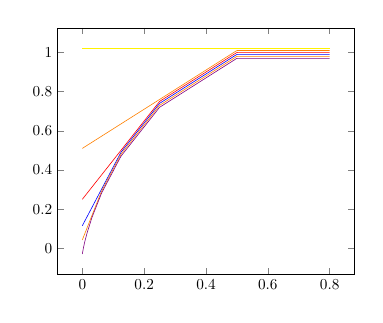
\begin{tikzpicture}[scale=0.55]
\begin{axis}[samples=250]
\addplot[yellow,domain=0:0.8] {1+0.02};

\addplot[orange,domain=0:0.8] {min(x+1/2, 1)+0.01};


\addplot[red,domain=0:0.8] {min(2*x+1/4, x+1/2, 1};
\addplot[blue,domain=0:0.8] {min(3*x+1/8,2*x+1/4, x+1/2, 1)-0.01};
\addplot[orange,domain=0:0.8] {min(4*x+1/16,3*x+1/8,2*x+1/4, x+1/2, 1)-0.02};

\addplot[violet,domain=0:0.8] {min(
10*x+1/1424,
9*x+1/712,
8*x+1/356,
7*x+1/128,
6*x+1/64,
5*x+1/32,
4*x+1/16,3*x+1/8,2*x+1/4, x+1/2, 1)-.03};


\end{axis}

\end{tikzpicture}
\caption{Plot of the tropical polynomials $\varphi_1,\varphi_2,\varphi_3,\varphi_4$ (from top to bottom), and of their limit tLs $\varphi$ (in violet).}
\label{fig:plot1}
%\end{figure} 
\end{wrapfigure} %%

\begin{proposition}\label{prop:nondecr+conc}
 Any tLs $f:\Lawv^X\to\Lawv^Y$ is non-decreasing and concave, w.r.t.\ the pointwise order.
\end{proposition}


%In Example~\ref{ex:famous_ex}, 
Look at Fig~\ref{fig:plot1}: it appears that $\varphi$ behaves \emph{locally} like the polynomials $\varphi_{n}$. 
%In particular, for all $\epsilon >0$, $f$ coincides on $[\epsilon,\infty]$ with some polynomial $\varphi_{n}$. More, precisely, $\varphi$ coincides with $\varphi_{n}$ for $\epsilon \geq 2^{-(n+1)}$, the smallest tropical root of $\varphi_{n}$.
However, at
%
%$x\in [\epsilon,\infty]$, with $\epsilon>0$
%It can be proven by hand that $\varphi(x)$ is a $\min$ for all $x>0$.
 $x=0$ we have that $\varphi(x=0)=\inf_{i\in\N} 2^{-i}=0$, and this is the only point where the $\inf$ is \emph{not} a $\min$.
Also, while the derivative of $\varphi$ is bounded on all $\BB R_{>0}$, at $x=0$ it tends to $\infty$.
This phenomenon is reminiscent of [Example 7, \cite{Ehrhard2005}],
%Differentials and Distances in Probabilistic Coherence Spaces. FSCD 2019
which actually motivated our first investigations.
In fact, these properties are shared by all tLs with \emph{finitely} many variables, as shown by the following result.


Remark that $!\set{1,\dots,k}$ can be identified with $\N^k$.
So the matrix of a tLs $f$ with finitely many variables $x=x_1,\dots,x_k$ (and one variable $f(x)$ in output) can be given as a $\matr f:\N^k\to\Lawv$, and $f$ has shape $f(x)=\inf_{n\in \N^k}\set{nx+\matr f(n)}$, where $nx$ is the scalar product.

\begin{theorem}\label{theorem:fepsilon}
 Let $k\in\N$ and $f:\Lawv^k\to\Lawv$ a tLs with matrix $\matr f:\N^k\to\Lawv$.
 For all $0<\epsilon<\infty$, there is a \emph{finite} $\C F_\epsilon \subseteq \N^k$ such that 
% 
% \begin{enumerate}
%  \item If $\C F_\epsilon=\emptyset$ then $f=\infty$ on all $\Lawv^k$;
%  \item If $f(x_0)=\infty$ for some $x_0\in[0,\infty)^k$, then $\C F_\epsilon=\emptyset$;
  %\item 
$f$ coincides on all $[\epsilon,\infty]^k$ with the tropical {polynomial} $P_\epsilon(x):=\min_{n\in \C F_\epsilon}\set{nx+\matr f(n)}$.
% \end{enumerate}
\end{theorem}
\begin{proof}[Proof sketch]
Let $\C F_\epsilon$ be the set of $n\in\N^{k}$ such that 
$\widehat f(n)<\infty$ and $\widehat f(m)> \widehat f(n)+\epsilon$ holds for all $m\prec n$, where $\preceq$ is the pointwise order on $\N^k$.
We can show that it is finite and does the job.
\end{proof}



The norm $\norm{\cdot}_\infty$ on $\BB R$ naturally induces a metric $\norm{x-y}_{\infty}$ over the spaces $\Lawv^{X}$.
We will show that tLs satisfy suitable Lipschitz properties  w.r.t.~these metrics.
\emph{Wlog}, we will often take $Y=\set{*}$. 

First, it can be seen that all tropical \emph{linear} functions $f: \Lawv^{X}\to \Lawv^{Y}$ are non-expansive.  
%\begin{proof}[Proof sketch]
%Using the fact that $f(\B x)_{b}= \inf_{a\in X}\matr f_{a,b}+\B x_{a}$,
%the problem reduces to checking that $|(\matr f_{a,b}-\B x_{a})- (\matr f_{a,b}-\B y_{a})| = |\B x_{a}-\B y_{a}|\leq \| \B x-\B y\|_{\infty}$.\end{proof}
This result shows that, in analogy with that happens in usual metric semantics, linear programs are interpreted by non-expansive functions. 
%\begin{proof}
%Using $f(\B x)_{b}= \inf_{a\in X}\matr f_{a,b}+\B x_{a}$,
%first observe that $|(\matr f_{a,b}-\B x_{a})- (\matr f_{a,b}-\B y_{a})| = |\B x_{a}-\B y_{a}|\leq \| \B x-\B y\|_{\infty}$; we now have
%$|f(\B x)_{b}-f(\B y)_{b}| \leq |(\inf_{a\in X}\matr f_{a,b}-\B x_{a})-(\inf_{a\in X}\matr f_{a,b}-\B y_{a})| \leq
%\sup_{a\in X}|(\matr f_{a,b}-\B x_{a})- (\matr f_{a,b}-\B y_{a})|\leq 
% \| \B x-\B y\|_{\infty}$.
%\end{proof}
Let us now consider the case of bounded exponentials:
\begin{proposition}\label{prop:boundedlip}
If a tLs $f: \Lawv^{X}\to \Lawv^{Y}$ arises from a bounded matrix $\matr f:!_{n}X\times Y\to \Lawv$, then $f$ is $n$-Lipschitz-continuous.
\end{proposition}
\begin{proof}[Proof sketch]
It follows from the above lines about tropical linear functions, plus the remark that, for all $x\in \Lawv^{X}$, $\norm{ !_{n} x-!_{n} y}_{\infty}\leq n\cdot \norm{ x- y}_{\infty}$, where $!_{n} x$ is the restriction of $! x$ to finite multisets of degree $\leq n$.%
%Using the fact that $f(\B x)_{b}=\inf_{\mu\in \C M_{\leq n}(X)}\{ \matr f_{\mu,b}+ \mu (!_{n}\B x) \}$, where $!_{n}\B x\in \Lawv^{\C M_{\leq n}(X)}$ is given by 
%$(!_{n}\B x)_{[a_{1},\dots, a_{k}]}=\sum_{i=1}^{k}\B x_{a_{i}}$, 
%it suffices to check that $\| (!_{n}\B x)-(!_{n}\B y)\|_{\infty}\leq n\cdot \| \B x-\B y\|_{\infty}$ and apply Proposition \ref{prop:troplinear}.
\end{proof}
This result is perfectly analogous to what happens in the metric models discussed in Section \ref{section2}, the bounded exponentials $!_{n}$ playing the role of the re-scaling trick.
It also entails that for any tropical polynomial $\varphi:\Lawv^{X}\to\Lawv$, $\varphi$ is $\mathrm{deg}(\varphi)$-Lipschitz continuous.


Let us now look at what happens with tLs, i.e.~when considering the full exponential $!$.
As consequence of Theorem~\ref{theorem:fepsilon}, the tLs with \emph{finitely many} variables are always \emph{locally} Lipschitz on all $\BB R_{>0}$.
Actually, we can prove a more general statement, also covering the infinitary case.


\begin{theorem}\label{thmTLSlocLip}
 All tLs $\Lawv^X\to\Lawv$ are locally Lipschitz on $\BB R_{>0}^X$.
\end{theorem}
\begin{proof}[Proof sketch]
The core of the proof is a convex analysis argument showing that an arbitrary function $f:\Lawv^X\to\Lawv$ which is non-decreasing, concave and continuous, must be locally Lipschitz. 
\end{proof}

Finally, the differential operator $D$ of $\LREL_{!}$ translates into a differential operator $D_{!}$ turing a tLs $f:\Lawv^{X}\to \Lawv^{Y}$ into a tLs $D_{!}f:\Lawv^{X}\times \Lawv^{X}\to \Lawv^{Y}$, linear in its first variable, and given by $D_{!}f(x,y)_{b}=\inf_{a\in X, \mu\in !X}\left\{\matr f_{\mu+a}+x_{a}+\mu y\right\}$.
One can check that, when $f$ is a tropical polynomial, $D_{!}f$ coincides with the standard tropical derivative (see e.g.~\cite{Grigoriev2017}).
Moreover, the Taylor formula enjoyed by $\LREL_!$ morphisms, yields a ``tropical'' Taylor formula for tLs of the form $f(x)=\inf_{n}\left\{D_{!}^{(n)}(f)(!_{n}x,\infty)\right\}$.


The above results translate into the following facts about the interpretation of higher-order programs:
\begin{corollary}\label{thm:main}
For any $\lambda$-term $M$:
\begin{enumerate}
\item if $\Gamma \vdash_{\BSTLC} M:A$, then $\model M^!:\model\Gamma \to \model A$ is a \emph{Lipschitz} map.
\item if $\Gamma \vdash_{\STLC}M:A$, then $\model M^!: \model\Gamma \to \model A$ is a \emph{locally Lipschitz} map.
\item  if $\Gamma \vdash_{\STLC}M:A$, then its Taylor exp.\ decomposes $\model M^!: \model\Gamma \to \model A$ into an $\inf$ of \emph{Lipschitz}~maps.
\end{enumerate}
\end{corollary}


\section{Relations to quantitative properties}



\section{Lawvere's generalised metric spaces}

We already remarked that the tropical semiring $\Lawv$ coincides with the \emph{Lawvere quantale} $\Lawv=([0,\infty], \geq, +)$.
In particular, a (possibly $\infty$) metric on a set $X$ is nothing but a ``$\Lawv$-valued square matrix'' $d:X\times X\to \Lawv$ satisfying axioms like e.g.~the triangular law (indeed, such distance matrices correspond to $\Lawv$-\emph{enriched categories}, a viewpoint we explicitly take in Section \ref{section6}). 

\begin{remark}
 The category $\QREL$ is (equivalent to) a subcategory of the category $Q\SF{Mod}$ of \emph{complete} $Q$-semimodules.
 If $\QREL$ corresponds to considering semimodules (the $Q^X$'s) whose vectors are given in coordinates w.r.t.\ a \emph{fixed base} (the set $X$), $Q\SF{Mod}$ corresponds to considering semimodules in abstract, without fixing a base.
 We take this viewpoint in Section~\ref{section6}.
\end{remark}


%The optional arguments of {\tt $\backslash$documentclass$\{$eptcs$\}$} are
%\begin{itemize}
%\item at most one of
%{\tt adraft},
%{\tt submission} or
%{\tt preliminary},
%\item at most one of {\tt publicdomain} or {\tt copyright},
%\item and optionally {\tt creativecommons},
%  \begin{itemize}
%  \item possibly augmented with
%    \begin{itemize}
%    \item {\tt noderivs}
%    \item or {\tt sharealike},
%    \end{itemize}
%  \item and possibly augmented with {\tt noncommercial}.
% \end{itemize}
%\end{itemize}
%We use {\tt adraft} rather than {\tt draft} so as not to confuse hyperref.
%The style-file option {\tt submission} is for papers that are
%submitted to {\tt $\backslash$event}, where the value of the latter is
%to be filled in in line 2 of the tex-file. Use {\tt preliminary} only
%for papers that are accepted but not yet published. The final version
%of your paper that is to be uploaded at the EPTCS website should have
%none of these style-file options.

%By means of the style-file option
%\href{http://creativecommons.org/licenses/}{creativecommons}
%authors equip their paper with a Creative Commons license that allows
%everyone to copy, distribute, display, and perform their copyrighted
%work and derivative works based upon it, but only if they give credit
%the way you request. By invoking the additional style-file option {\tt
%noderivs} you let others copy, distribute, display, and perform only
%verbatim copies of your work, but not derivative works based upon
%it. Alternatively, the {\tt sharealike} option allows others to
%distribute derivative works only under a license identical to the
%license that governs your work. Finally, you can invoke the option
%{\tt noncommercial} that let others copy, distribute, display, and
%perform your work and derivative works based upon it for
%noncommercial purposes only.

%Authors' (multiple) affiliations and emails use the commands
%{\tt $\backslash$institute} and {\tt $\backslash$email}.
%Both are optional.
%Authors should moreover supply
%{\tt $\backslash$titlerunning} and {\tt $\backslash$authorrunning},
%and in case the copyrightholders are not the authors also
%{\tt $\backslash$copyrightholders}.
%As illustrated above, heuristic solutions may be called for to share
%affiliations. Authors may apply their own creativity here \cite{multipleauthors}.



%\section*{Bibliography}

%We request that you use
%\href{http://eptcs.web.cse.unsw.edu.au/eptcs.bst}
%{\tt $\backslash$bibliographystyle$\{$eptcs$\}$}
%\cite{bibliographystylewebpage}, or one of its variants
%\href{http://eptcs.web.cse.unsw.edu.au/eptcsalpha.bst}{eptcsalpha},
%\href{http://eptcs.web.cse.unsw.edu.au/eptcsini.bst}{eptcsini} or
%\href{http://eptcs.web.cse.unsw.edu.au/eptcsalphaini.bst}{eptcsalphaini}
%\cite{bibliographystylewebpage}. Compared to the original {\LaTeX}
%{\tt $\backslash$biblio\-graphystyle$\{$plain$\}$},
%it ignores the field {\tt month}, and uses the extra bibtex fields {\tt eid}, {\tt doi}, {\tt ee} and {\tt url}. The first is for electronic identifiers (typically the number $n$ indicating the $n^{\rm th}$ paper in an issue) of papers in electronic journals that do not use page numbers. The other three are to refer, with life links, to electronic incarnations of the paper.

%\nocite{*}
%\bibliographystyle{eptcs}
%\bibliography{generic}

%\bibliographystyle{plain}
%\bibliography{tropical.bib}

\end{document}